%%%% Paramétrage du TD %%%%
\def\xxactivite{Colle 02 \ifprof -- Corrigé \else \fi} % \normalsize \vspace{-.4cm}



\def\xxtitreexo{Porte-outil}
\def\xxsourceexo{\hspace{.2cm} \footnotesize{Équipe PT -- PT$\star$ La Martinière Monplaisir}}
\def\xxauteur{\textsl{Xavier Pessoles}}


\def\xxcompetences{%
\vspace{.25cm}
\textsl{%
\textbf{Savoirs et compétences :}
\begin{itemize}[label=\ding{112},font=\color{ocre}] 
\item \textit{C2-08} :Déterminer les actions mécaniques en dynamique dans le cas où le mouvement est imposé.
\end{itemize}
}}
\def\xxfigures{
%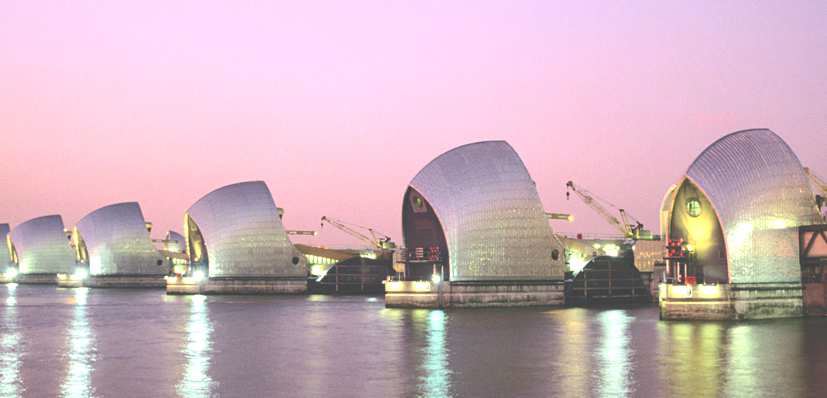
\includegraphics[width=.7\linewidth]{fig_00}
}%figues de la page de garde


\input{\repRel/Style/pagegarde_TD}
\setcounter{numques}{0}

\setlength{\columnseprule}{.1pt}

\pagestyle{fancy}
\thispagestyle{plain}

\vspace{5.1cm}

\def\columnseprulecolor{\color{ocre}}
\setlength{\columnseprule}{0.4pt} 

%%%%%%%%%%%%%%%%%%%%%%%

\setcounter{exo}{0}

\ifprof
\else
\begin{multicols}{2}
\fi


Soit le rotor \textbf{(1)} défini ci-dessous. Il est constitué d'un arbre de masse négligeable en liaison pivot par rapport à un bâti \textbf{(0)}. Sur cet arbre est monté, en liaison complète, un disque de masse $M$, de rayon $R$ et d'épaisseur $H$. 
Le repère $\mathcal{R}'_1=\repere{G}{x_1'}{y_1'}{z_1'}$ est attaché à ce solide.

La base $\mathcal{B}'_1=\base{x_1'}{y_1'}{z_1'}$ se déduit de $\mathcal{B}_1=\base{x_1}{y_1}{z_1}$  par une rotation d'angle $\alpha$ autour de $\vect{z_1}= \vect{z_1'}$. 

La base $\mathcal{B}_1=\base{x_1}{y_1}{z_1}$ se déduit de $\mathcal{B}_0=\base{x_0}{y_0}{z_0}$  par une rotation d'angle $\theta$ autour de $\vect{x_1}= \vect{x_0}$. 

Enfin, le rotor \textbf{1} est entrainé par un moteur (non représenté) fournissant un couple noté $C_m\vect{x_0}$. 
Le montage de ce disque présente deux défauts :
\begin{itemize}
\item un défaut de perpendicularité caractérisé par l'angle $\alpha$ ;
\item un défaut d'excentricité représenté par la cote $e$.
\end{itemize}


\begin{center}
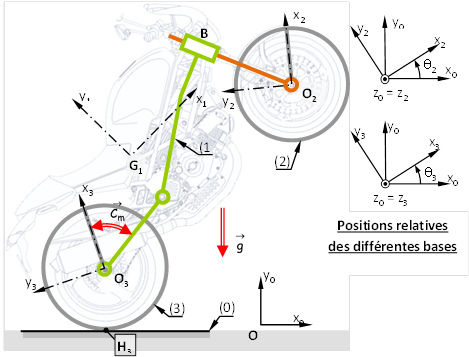
\includegraphics[width=\linewidth]{fig_01}
\end{center}
\begin{center}
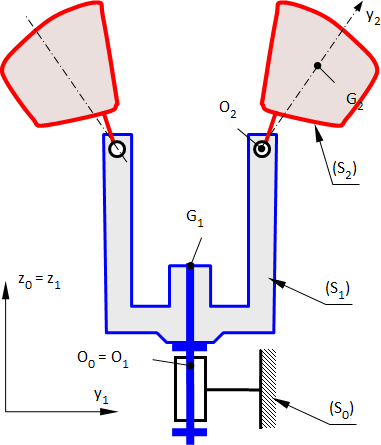
\includegraphics[width=\linewidth]{fig_02}
\end{center}

\question{Déterminer la forme de la matrice d'inertie dy cylindre en C dans la base $\mathcal{B}_1'$.}

\question{Déterminer les éléments de réduction en $A$ du torseur dynamique de \textbf{(1)} dans son mouvement par rapport à $\mathcal{R}_0$.}

\question{Appliquer le PFD pour déterminer les inconnues de liaison.}

\ifprof
\else
\end{multicols}
\fi



\ifprof
\begin{center}
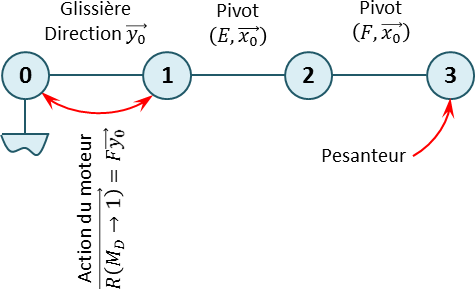
\includegraphics[width=\linewidth]{cor_01}
\end{center}
\begin{center}
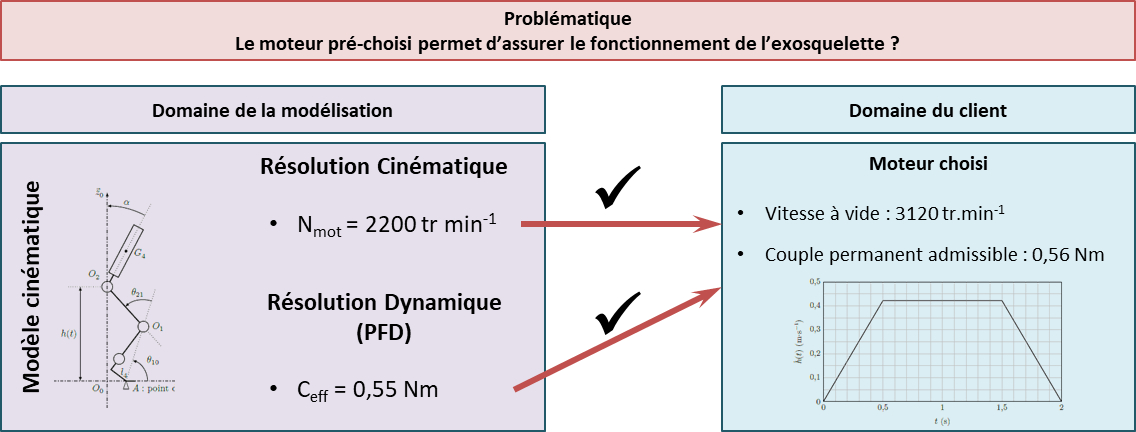
\includegraphics[width=\linewidth]{cor_02}
\end{center}
\begin{center}
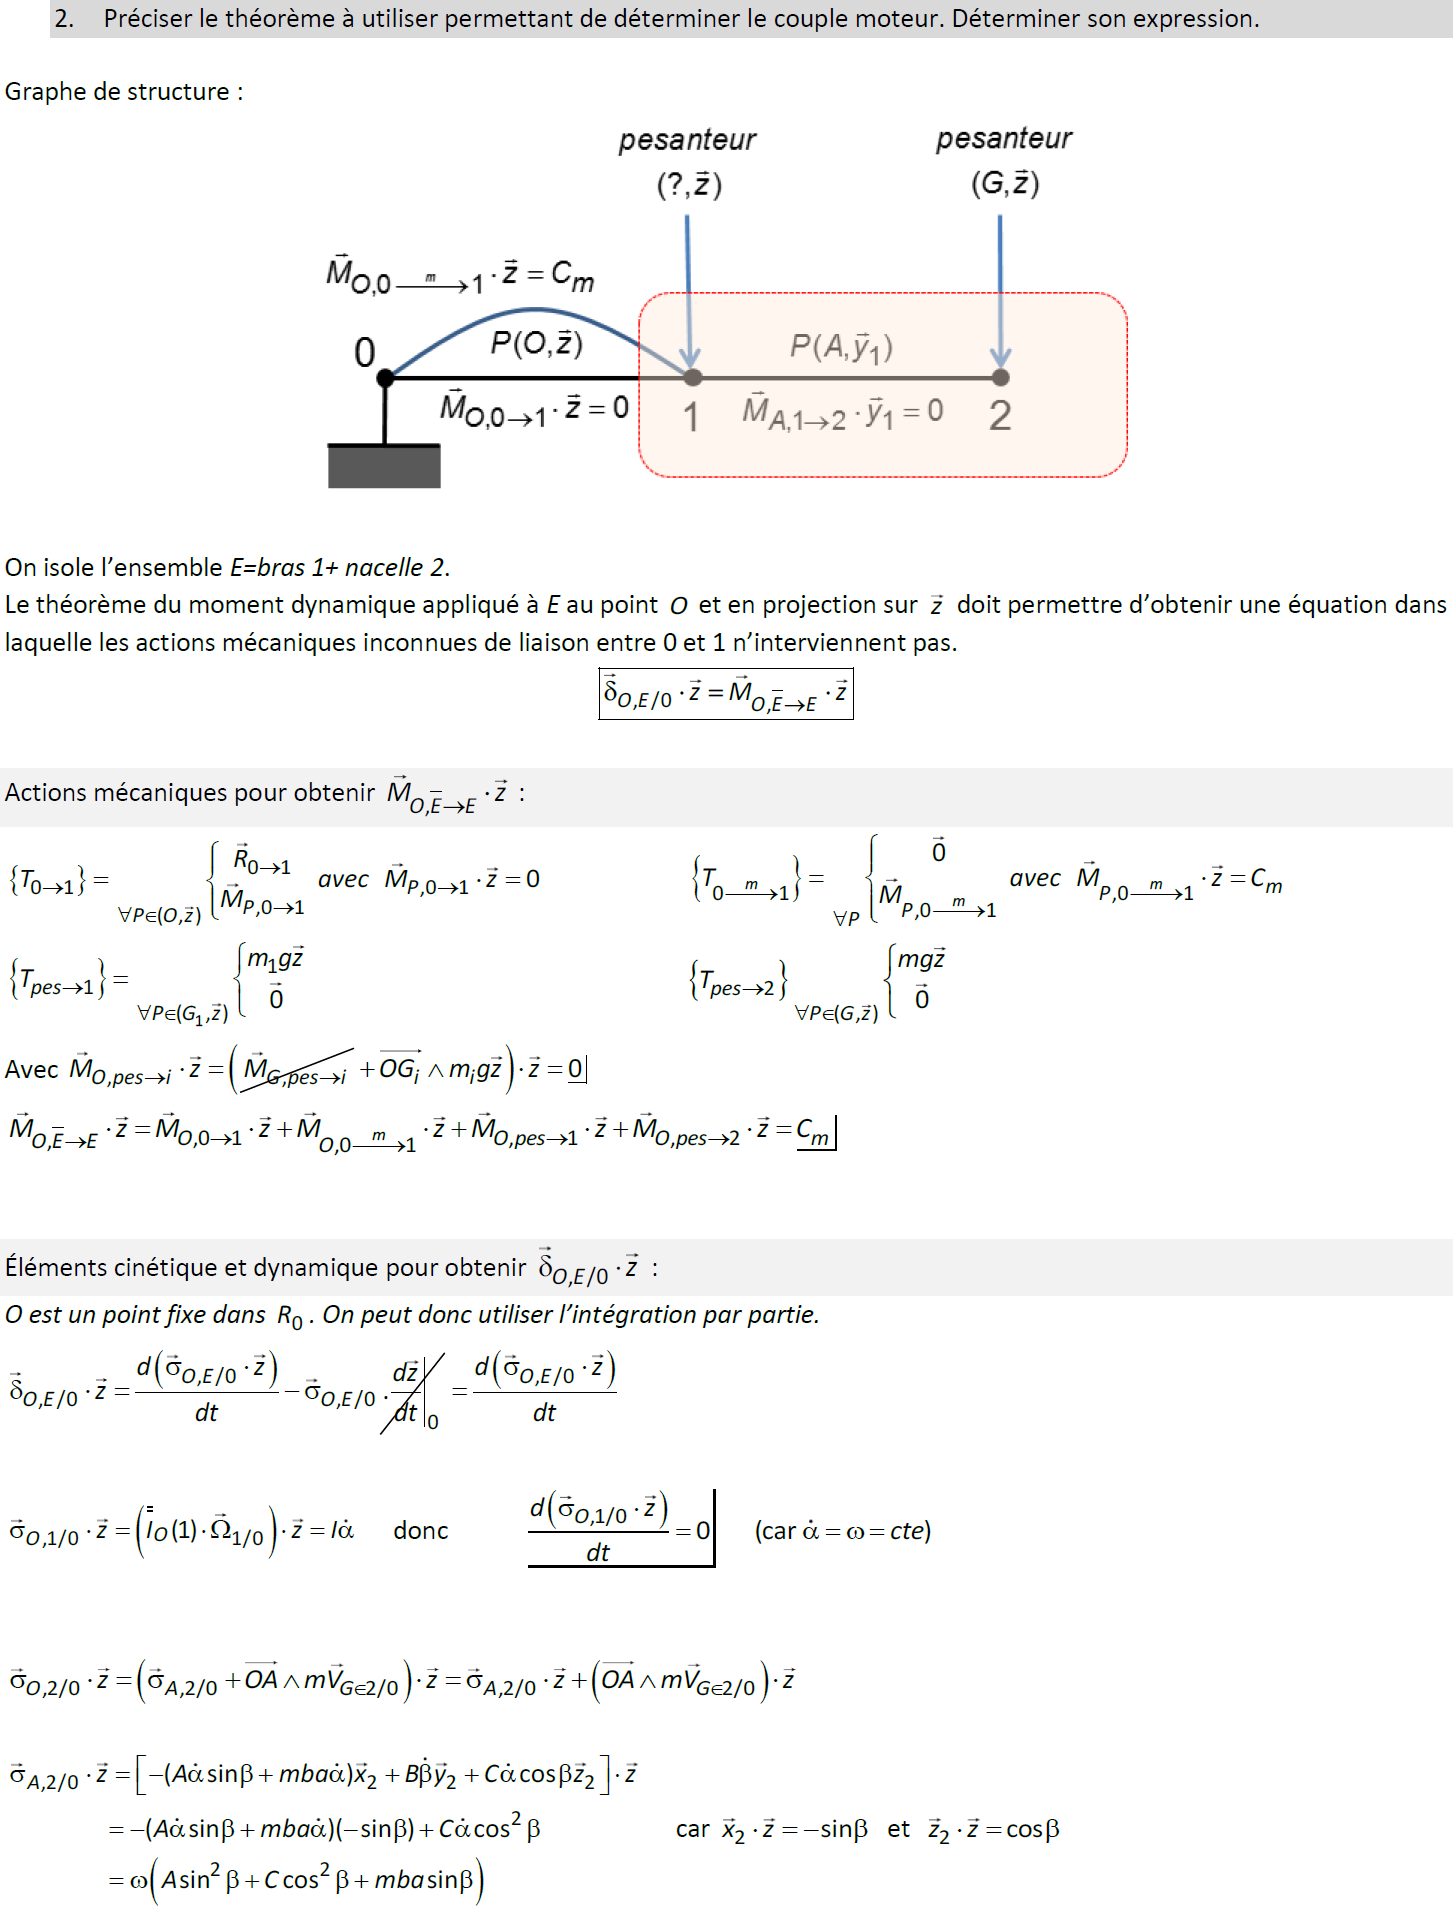
\includegraphics[width=\linewidth]{cor_03}
\end{center}
\begin{center}
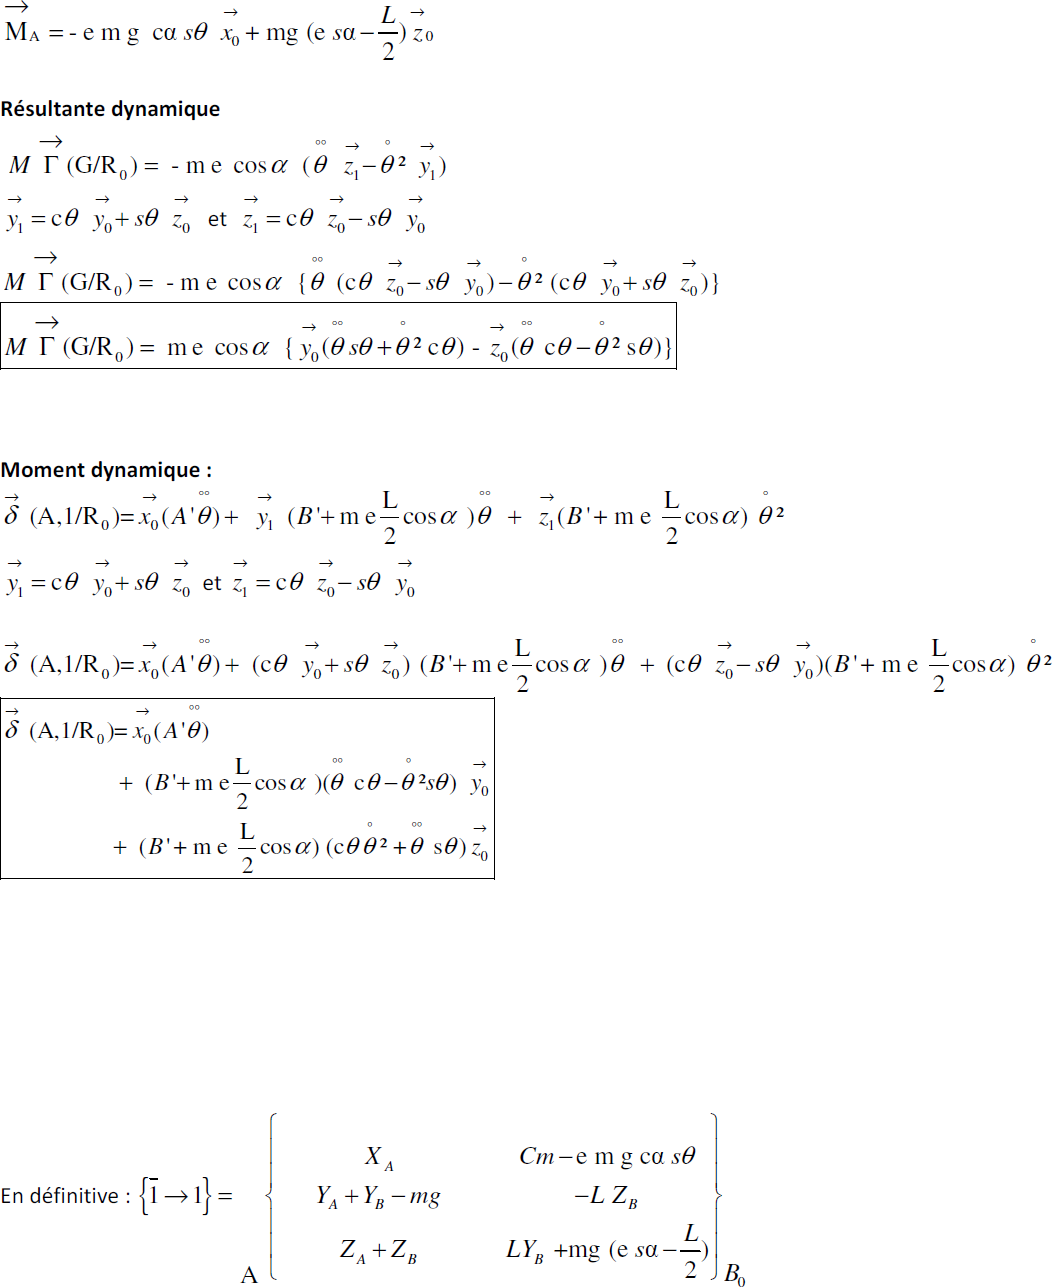
\includegraphics[width=\linewidth]{cor_04}
\end{center}
\begin{center}
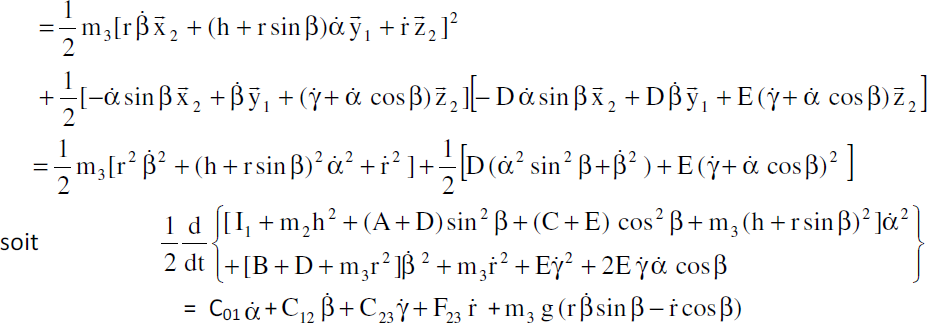
\includegraphics[width=\linewidth]{cor_05}
\end{center}

\else
\fi

